Im folgenden Kapitel werden die Grundlagen von Domain Specific Languages aufgearbeitet. 
Zuerst wird versucht, eine genaue Definition f"ur den Begriff DSL zu finden. 
Anhand von Beispielen wird gezeigt, wie flexibel dieser Begriff verwendet werden kann. 
Danach werden die Grundlagen von formalen Sprachen herausgearbeitet, die f"ur das Verst"andnis der Arbeit von Bedeutung sind. 
Ein weiteres Kapitel widmet sich den verschiedenen Tools, die das Erstellen von Sprachen unterstützen können und geht insbesondere auf das Werkzeug der Wahl, ANTLR, ein.
Das Ende des ersten Teils dieser Arbeit widmet sich dem Wissenschaftlichen Umfeld und gibt einen Überblick über weitere Arbeiten und Ansätze.



\newpage

\chapter{Domain Specific Languages}
\label{chapter_dsl}

Dieser Abschnitt beschreibt, was eine DSL ist, vergleicht die Vor-, Nachteile und Unterschiede zu General Purpose Languages (GPL), versucht eine für die vorliegende Arbeit geeignete Definition zu finden und gibt Beispiele für bekannte DSLs.

\section{Definitionen}

Dem Begriff Domain Specific Language steht der der General Purpose Language gegenüber. Mit GPLs lassen sich viele unterschiedliche Problemstellungen lösen, die nicht auf eine Branche oder einen Einsatzbereich beschränkt sind. Bekannte Programmiersprachen, die der Kategorie der GPLs zugerechnet werden, sind beispielsweise Java, C/++/\#, Python etc. Mit Domäne, oder auch Anwendungsdomäne wird ein abgegrenzter Einsatzbereich bezeichnet, der für diesen charakteristische, bzw. eben domänenspezifische, Anforderungen an ein System stellt.

Eine genaue Definition für den Begriff DSL zu finden ist nicht einfach, da die Bezeichnung in der wissenschaftlichen Community im Moment sehr inflationär gebraucht wird\footnote{Bevor sich der Begriff DSL etablierte, wurden domänenspezifische Sprachen oft als ``little languages'' bezeichnet., \cite{VaDe00}}. Eine kompakte Definition einer DSL gibt Martin Fowler in \cite{Fowl05}:

\begin{myquote}
Domain-specific language (noun): a computer programming language of limited expressiveness focused on a particular domain.
\end{myquote}

Eine sehr ähnliche, aber detailliertere Definition kommt von Mernik et al. \cite{MeHe05}:

\begin{myquote}
Domain-specific languages (DSLs) are languages tailored to a specific application domain. They offer substantial gains in expressiveness and ease of use compared with general-purpose programming languages in their domain of application.
\end{myquote}


Ein Unterschied, der ins Auge sticht, ist, dass Fowler die eingeschränkte Ausdrucksstärke ("limited expressiveness") betont, Mernik et al. aber den erheblichen Gewinn an Ausdrucksstärke ("'substantial gains in expressiveness"). Fowler meint damit, dass man durch die Fokussierung auf eine Domain eine Einschränkung des Einsatzbereiches erzwingt. Mernik et al. sehen den Gewinn an Ausdrucksstärke darin, dass mit einem einzelnen Statement in einer DSL mehr ausgesagt werden kann, als mit einem Statement einer GPL, das DSL-Statement ist also ausdrucksstärker.

Die zweite Definition geht im Unterschied zur ersten auf zwei essentielle Eigenschaften ein: Erstens muss eine DSL genau auf eine bestimmte Domain zugeschnitten sein und zweitens muss sie im Gegensatz zu einer GPL im spezifischen Einsatzbereich einfacher anzuwenden sein.

Ein Grund, warum Fowler in seiner Definition auf die Einfachheit im Gegensatz zu einer allgemeinen Programmiersprache verzichtet, mag seine Einteilung in interne und externe DSLs \cite{FoPa10} sein\footnote{Die Klassifikation in interne und externe DSLs ist nicht die einzige. So können sie auch nach Features oder Darstellungsart (textuell, tabellarisch, graphisch etc.) eingeteilt werden. \cite{LaJi07} }:

\subsection{Interne DSL}

Interne DSLs benutzen die Syntax und die Laufzeitumbgebung einer GPL. Oft wird unter der Bezeichnung interner (bzw. embedded) DSL eine entsprechende API für eine spezifische Domäne verstanden\footnote{Oft wird in diesem Zusammenhang Bjarne Stroustrup, der Entwickler von C++, zitiert: "Library design is language design"'}.
Das Problem ist das Mapping des domainspezifischen Problems auf eine GPL. Eine sehr beliebte Möglichkeit, APIs eine gewisse ``sprachähnlichkeit'' zu verabreichen, ist das sogenannte Method Chaining
\cite{RuBa08}.
Bei dieser Technik wird das Objekt, auf dem eine Methode aufgerufen wird, von ebendieser Methode wieder zurückgegeben. So können Methodenaufrufe verkettet werden, was sehr intuitive Statements zur Folge haben kann.

In manchen Sprachen können Sprachfeatures verwendet werden, um die Sprache zu einer eigenen DSL zu erweitern. Die Sprache JavaScript bietet etwa die Möglichkeit, Typen und Objekte zur Laufzeit dynamisch zu verändern (Listing \ref{listing_javascript_each}).\\

\begin{lstlisting}[language=JavaScript, caption={Erweiterung des Array-Typs um die Funktion \texttt{each()} in der JavaScript Bibliothek Prototype},label=listing_javascript_each]
['1', '2', '3'].each(function(elem){
	alert('Number ' +elem);
});
\end{lstlisting}

Eine weitere Möglichkeit, eine interne DSL zu verwenden, bietet die Einbindung einer Laufzeitumgebung einer allgemeinen Programmiersprache in ein Softwaresystem. Eine Methode bietet die Java Plattform mit der Einbettung von verschiedenen Script-Engines(vgl. Abschnitt \ref{section_java_scripting}).

\subsection{Externe DSL} 

Da externe DSLs nicht eingebettet in einer anderen Sprache ausgeführt werden, ist eine eigene Laufzeitumbebung notwendig. 

Eine externe DSL ist als individuelle Sprache mit eigener Syntax definiert, die allerdings auch existierende Notationen verwenden kann. Zusätzlich zur frei definierten Syntax, muss auch die Semantik explizit definiert werden. Der große Unterschied zu internen DSLs ist, dass die Komplexität der Sprache genau auf die Domäne, für die sie verwendet wird, beschränkt werden kann. Die Erstellung von Interpretern und Übersetzern wird durch eine Vielzahl meist freier Werkzeuge unterstützt.

In der Entscheidungsphase beim Design der DSL zur Berechnung und Evaluierung von Formularfeldern wird nochmals genauer 
auf das Thema interne vs. externe DSLs und deren Vor- und Nachteile im Bezug auf die Aufgabenstellung dieser 
Arbeit eingegangen (Kapitel \ref{chapter_entscheidung}).

Weiters führt Fowler auch noch \textit{Language Workbenches} als eigene Kategorie domänenspezifischer Sprachen auf. 
Darunter versteht man hochintegrierte Entwicklungsumgebungen, die nicht nur die Definition und Generierung von DSLs ermöglichen, 
sondern auch eine Entwicklungsumgebung für die erstellte Sprache zur Verfügung stellen
\footnote{Eine der bekanntesten Language Workbenches ist Jetbrains's MPS. Eine Übersicht über Language Workbenches und eine 
Vergleichsmatrix findet sich unter http://www.languageworkbenches.net/index.php?title=LWC2011\_Comparison\_Matrix, 20.12.2011}.



\section{Vorteile und Nachteile}

Wie bereits erwähnt, können domänenspezifische Sprachen einen erheblichen Gewinn an Produktivität und Wartbarkeit mit sich bringen\cite{VaDe98}. DSLs sind für den Endbenutzer besser zu handhaben. Durch die domänenspezifische Notation und der damit einhergehenden besseren Les- und Schreibbarkeit ist es für Domänenexperten leichter, die Sprache zu verwenden. 

Ein weiterer großer Vorteil ist die Validierung und Optimierung der Sprache auf Domain-Level. Das bedeutet, dass dem Benutzer viel detaillierter Feedback über die eingegebenen Programme und eventuell auftretende Fehler gegeben werden kann, als es eine allgemeine Programmiersprache könnte\cite{VaDe00}.

DSLs haben nicht nur Vorteile, sondern auch Nachteile und Einschränkungen. Ein Nachteil ist der notwendige Entwicklungsaufwand, um die Sprache zu erstellen. Der Aufwand, der zuerst investiert werden muss, benötigt einen entsprechenden Zeitraum, um sich zu amortisieren.

Die domänenspezifische Notation kann sich auch als Nachteil erweisen, weil sie die Möglichkeiten dahingehend einschränkt, dass wirklich nur die dafür vorgesehenen Aufgaben erledigt werden können. Statt einer Erweiterung der Funktion wie in GPLs durch eigene Klassen und Funktionen ist bei einer DSL eine Änderung der Sprachdefinition und der Laufzeitumgebung notwendig.

Einen weiteren Nachteil kann der Verlust von Performance und Effizienz einer selbst erstellten DSL im Vergleich zu einer ausgereiften GPL darstellen\cite{VaDe00}.



\section{Beispiele}
\label{grundlagen_examples}

Es finden sich diverse Beispiele für Sprachen, die auf einen eigenen Anwendungsbereich zugeschnitten sind. Nachfolgend werden einige Beispiele vorgestellt, die sich in der Informatik etabliert haben.

\paragraph*{SQL}
(Structured Query Language) ist eine Sprache zur Abfrage und Manipulation von Daten in relationalen Datenbanken. Sie eignet sich sehr gut als Beispiel für eine DSL, da sie die wesentlichen Eigenschaften hat: eine eigene, genau spezifizierte Domäne (Definition, Abfrage, Manipulation von Daten(banken)) und eine eingeschränkte Syntax, die auf die von GPLs bekannten Konstrukte wie Schleifen verzichtet.

\paragraph*{\LaTeX} ist ein Softwarepaket zum setzen von Texten, das auf der Software \TeX \ aufbaut. Im Gegensatz zu herkömmlichen Textverarbeitungswerkzeugen werden Texte in Latex nicht in einem graphischen Editor bearbeitet, sondern in einem einfachen Textdokument. Elemente wie Überschriften oder Bilder werden im Text mit einfachen Befehlen ausgezeichnet. Das Latex-Dokument kann dann in verschiedene Formate, wie Postscript, PDF oder HTML ausgegeben werden. Wie HTML is Latex also keine Programmiersprache, sondern eine Auszeichnungssprache.


\paragraph*{EBNF}
(Extended Bacus-Naur Form) ist - wie der Name vermuten lässt - eine Erweiterung der Bacus-Naur Form. Sie ist eine Metasprache zur Definition von Grammatiken und erlaubt die Darstellung von Produktionsregeln, Nichtterminalsymbolen und Terminalsymbolen in einer leicht verständlichen Form\cite{NiWi77}. Sie definiert Wiederholungen in geschweiften, und optionale Elemente in eckigen Klammern. Alternativen werden durch einen senkrechten Strich getrennt. 

\begin{lstlisting}[float = htbp,caption={Beschreibung eines Fließkomma-Typs in EBNF.},label=listing_example_ebnf]
DECIMAL = {DIGIT} "." DIGIT {DIGIT} | DIGIT {DIGIT} "." {DIGIT};

DIGIT   = "0"|"1"|"2"|"3"|"4"|"5"|"6"|"7"|"8"|"9" ;
\end{lstlisting}

Listing \ref{listing_example_ebnf} Beschreibt einen Fließkomma-Typ DECIMAL mit Hilfe der EBNF. Dieser Typ besteht aus beliebig vielen Ziffern vor und nach dem Kommapunkt, wobei jedoch zu beachten ist, dass mindestens eine Ziffer vor oder nach dem Kommapunkt verpflichtend ist.

Viele Tools zur Generierung von Parsern verwenden eine Abwandlung oder Erweiterung der EBNF zur Beschreibung der Grammatik (vgl. Abschnitt \ref{tools_vergleich}).




\chapter{Theoretische Grundlagen}

\label{chapter_theoretische_grundlagen}

In diesem Kapitel werden die theoretischen Grundlagen, die zum Verständnis der Arbeit notwendig sind aufbereitet. Diese beinhalten zunächst eine Übersicht über die anerkannten Methoden des Übersetzerbaus. Danach folgt eine Einführung in Formale Sprachen, die durch bestimmte Grammatiken erzeugt werden. Das ist vor allem deshalb notwendig, um ein Verständnis für die Arbeitsweise von Parsern zu erlangen. Weiters wird auf tiefere Konzepte wie Variablen und Funktionsaufrufe sowie den Umgang mit verschiedenen Datentypen eingegangen.


\section{Language Applications}
\label{theorie_language_applications}

Terence Parr definiert Language Applications nicht nur als Implementierung einer Sprache, sondern ``any program that processes, analyzes, or translates an input file''\cite{Parr10}. Diese allgemeine Definition ist vor allem für DSLs interessant, da diese of mehr  einer Konfigurationssprache als einer richtigen Programmiersprache ähnlich sind. Für das Auswerten von derart eingeschränkten Sprachen ist somit auch nicht unbedingt der volle Umfang eines Parsers, Interpreters oder Übersetzers im klassischen Sinne notwendig. Im Kontext dieser Arbeit wird nur ein Teil dieser Definition betrachtet, nämlich die Interpretation (im Sinne von Auswertung) von Ausdrücken, in Hinsicht auf erweiterte Konzepte von allgemeinen Language Applications. Darunter fallen in erster Hinsicht Variablen, Funktionen und Datentypen, die in der DSL verwendet werden sollen.

Der klassische Aufbau einer Language Application, wie er auch in diversen Lehrbüchern und Skripten zum Thema Compilerbau beschrieben ist, besteht aus den 4 Phasen lexikalische Analyse, syntaktische Analyse, semantische Analyse, Codeerzeugung, wobei im Falle einer interpretierten Sprache an Stelle der Codeerzeugung ein Laufzeitsystem tritt(Abbildung \ref{abb_language_application_klassisch})\footnote{Bei manchen interpretierten Sprachen wird zuerst Zwischencode erzeugt, der dann vom Interpreter abgearbeitet wird. Auch der AST (Abbildung \ref{abb_ast_vs_cst}) kann als Zwischencode betrachtet werden.}.


\begin{figure}[h]
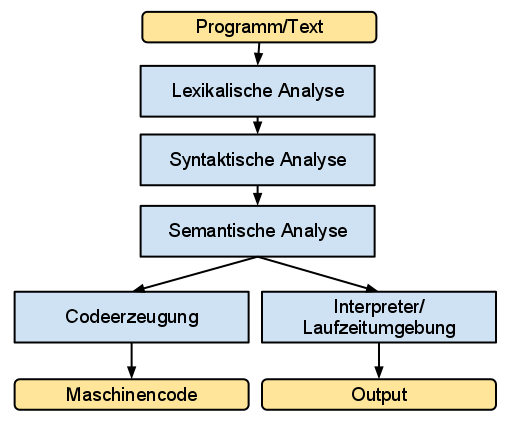
\includegraphics[width=\textwidth,scale=0.5]{figures/language_application_klassisch.png}
\caption{Klassischer Aufbau einer Language Application: Compiler (linker Zweig) und Interpreter (rechter Zweig)}
\label{abb_language_application_klassisch}
\end{figure}

In der Lexikalischen Analyse wird das Programm eingelesen und in Tokens\footnote{Oft wird in der deutschsprachigen Literatur das Wort Symbol synonym verwendet.} aufgeteilt. Ein Token ist ein Paar bestehend aus einem Bezeichner oder Typ und einem optionalen Wert\cite[S. 111ff]{AhSe86}. Tokens können Keywords und Operatoren einer Sprache, Bezeichner von Funktionen und Variablen oder Literale sein. Im Zuge der lexikalischen Analyse können auch Zeichen wie Tabulatoren oder Leerzeichen, sofern diese für die Weiterverarbeitung nicht interessant sind, verworfen werden. Die Ausgabe nach dieser Phase ist eine Folge von Tokens, die von der syntaktischen Analyse für das Parsing verwendet wird.

Beim Parsing (Syntaktische Analyse) wird versucht, die Tokenfolge den Regeln der zugrundeliegenden Grammatik unterzuordnen. So kann überprüft werden, ob die Eingabe der Syntax der Sprache entspricht. Verschiedene Strategien des Parsens werden in Abschnitt \ref{theorie_parsing_strategien} beschrieben. 

Das Ergebnis der Syntaktischen Analyse kann in einem Parse Tree dargestellt werden. Dabei wird zwischen den Formaten Concrete Syntax Tree(CST) und Abstract Syntax Tree(AST) unterschieden (Abbildung \ref{abb_ast_vs_cst}). Der CST gibt die der Syntax der Sprache entsprechende Hierarchie der Tokens, die bei der Lexikalischen Analyse identifiziert werden, wieder. Für die Darstellung des AST weren jene Tokens eleminiert, die durch die Struktur des Baumes ihre Bedeutung verlieren\footnote{Im Beispiel in der Abbildung werden etwa die Klammern vor und nach der Addition obsolet, da diese in einem eigenen Subtree dargestellt wird.}.  

\begin{figure}[h]
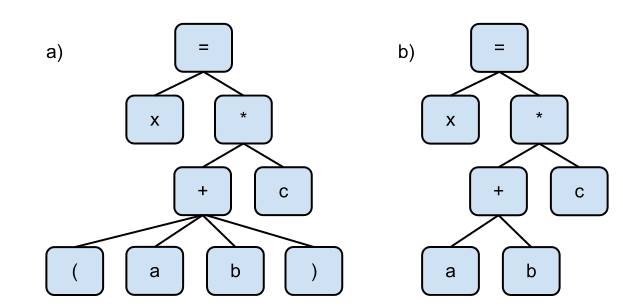
\includegraphics[width=\textwidth,scale=0.5]{figures/ast_vs_cst.png}
\caption{Vergleich der Parse Tree Formate a) Concrete Syntax Tree(CST) und b) Abstract Syntax Tree(AST) für den Ausdruck x=(a+b)*c}
\label{abb_ast_vs_cst}
\end{figure}

Die Semantische Analyse überprüft Anforderungen an das Programm, die nicht durch die Syntax abgedeckt werden können. Das betrifft vor allem die Überprüfung, ob ein Programm dem Typsystem entspricht. Das Typsystem setzt sich zusammen aus der Definition der vorhandenen Datentypen und den Regeln zur Zuweisung der Typen zu Operatoren (vgl. \cite[S. 426]{AhSe86}). In vielen Programmiersprachen sind einige Operatoren überladen, d.h. sie können mit verschiedenen Datentypen verwendet werden. In der Phase der semantischen Analyse werden die Rückgabetypen aus dem Kontext abgeleitet. Die Typen von Variablen und Funktionen können aus einer Symboltabelle ausgelesen werden, in der Deklarationen derselben gesammelt werden.

Je nach Einsatzzweck wird die Eingabe dann in Maschinencode übersetzt oder in einer Laufzeitumbebung ausgeführt. Beim Compiler ist zu beachten dass die Codeerzeugungsphase in die Phasen Zwischencodeerzeugung, Codeoptimierung und Codeerzeugung aufgeteilt werden kann. 

Um den Rahmen der Arbeit nicht zu sprengen möchte ich hier zum tieferen Verständnis der einzelnen Phasen auf das Standardwerk \emph{Compilers: principles, techniques and tools} \cite{AhSe86} verweisen.


\section{Grammatiken}

Um die Syntax einer Sprache festzulegen ist eine formale Grammatik notwendig. Eine formale Grammatik $G \ = (\Sigma,\ N\ ,P\ ,S\ )$ besteht aus einer Menge von Terminalsymbolen $\Sigma$, einer Menge von Nichtterminalsymbolen $N$, den Produktionsregeln $P$, sowie dem Startsymbol $S$\footnote{Eine übersichtliche Einführung in die verschiedenen Grammatiken, sowie deren Unterschiede, Anwendungen und Normalisierungen, findet man in \cite{VoWi02}.}.

Eine Grammatik beschreibt die Menge aller syntaktisch korrekten Programme einer Sprache. Diverse Sprachen in unterschiedlichen Anwendungen erfordern unterschiedliche Typen von Grammatiken. Eine beliebte Einteilung wurde von Noam Chomsky in der sogenannten Chomsky-Hierarchie vorgenommen:

\begin{myquote}DEFINITION 6. For i = 1, 2, 3, a type i grammar is one meeting restriction i, and a type i language is one with a type i grammar. A type 0 grammar (language) is one that is unrestricted. 
Type 0 grammars are essentially Turing machines; type 3 grammars, finite automata. Type 1 and 2 grammars can be interpreted as systems of phrase structure description. \cite{Chom59}
\end{myquote}

Chomsky definiert also 4 Typen von Grammatiken, die unterschiedlich restriktive Ableitungsregeln haben:

\begin{itemize}
  \item Typ-0 Grammatiken: Dieser Typ repräsentiert die Menge aller formalen Grammatiken.
  \item Typ-1 Grammatiken: Grammatiken vom Typ 1 werden kontextsensitive Grammatiken genannt.
  \item Typ-2 Grammatiken: Dieser Typ definiert die kontextfreien Grammatiken. Die Syntax der meisten Programmiersprachen kann durch eine kontextfreie Grammatik beschrieben werden.
  \item Typ-3 Grammatiken: Diese sind jene Grammatiken, die durch reguläre Ausfrücke beschrieben werden können.
\end{itemize}

Der für Programmiersprachen relevante Typ ist also die Typ-2 bzw. kontextfreie Grammatik. Diese zeichnen sich dadurch aus, dass auf der linken Seite jeder Produktionsregel genau ein Nichtterminalsymbol steht (also ``frei von Kontext''). Auf der rechten Seite kann jede mögliche Folge von Terminal- bzw. Nichtterminalsymbolen stehen.



Meistens wird die Grammatik einer Sprache in einer Form dargestellt, die der Erweiterten Backus-Naur Form (EBNF, siehe Abschnitt \ref{grundlagen_examples}) ähnlich ist. In dieser Form sind die verschiedenen Bestandteile der Grammatik der Sprache (Terminal- bzw. Nichtterminalsymbole, Startsymbol und Produktionsregeln) gut ersichtlich und einfach nachzuvollziehen.

Je nach Parsingalgorithmus unterliegen die Grammatiken bestimmten Regeln, um vom Parser verarbeitet werden zu können.


\section{Parsing Strategien}
\label{theorie_parsing_strategien}

Ein Parser ist, allgemein gesprochen, ein Programm oder eine Softwarekomponente, die eine Eingabe in ein weiter verarbeitbares Format umwandelt. Es gibt verschiedene Ansätze, wie diese Aufgabe erfüllt werden kann. Grund\-sätz\-lich ist es möglich, eine Eingabe Top-Down oder Bottom-Up zu verarbeiten.

\subsection{Top-Down Analyse}

Bei der Top-Down Analyse wird versucht, ausgehend vom Startsymbol Ab\-lei\-tun\-gen zu finden, mit denen das gegebene Wort eingelesen werden kann. Dazu muss eine Tabelle erstellt werden, die jedem Eingabesymbol die ent\-sprech\-en\-de Produktionsregel zuordnet. Die Eingabe wird dann von links nach rechts mittels Linksableitungen abgearbeitet. Die Menge der Grammatiken, die mit dieser Methode verarbeitet werden können, werden LL(k) Grammatiken genannt. Das \emph{k} steht für den Lookahead, der notwedig ist, wenn einem Eingabesymbol mehrere Regeln in der Tabelle zugeordnet werden.


\subsection{Bottom-Up Analyse}

Die Bottom-Up Analyse geht den umgekehrten Weg, von der Tokenfolge zum Startsymbol. Sie versucht, in einer Eingabe eine Struktur zu finden, die den syntaktischen Regeln der Sprache entspricht. Nach und nach werden, abhängig vom Lookahead, ein oder mehrere Symbole eingelesen und davon ausgehend eine Produktionsregel aufgelöst.


\subsection{Erweiterte Konzepte und Optimierungen}
\label{theorie_erweiterte_konzepte}

\subsubsection{Backtracking} 

Unter Backtracking versteht man das Ausprobieren verschiedener Alternativen bei mehrdeutigen Produktionsregeln. Wenn eine Ableitung fehlschlägt, wird die Eingabe bis zur letzten Kreuzung zurückgespult und die nächste Alternative versucht. Erst wenn alle Alternativen erschöpft sind, wird ein Fehler zurückgegeben. Backtracking kann sehr aufwendig sein, da einzelne Regeln für eine Eingabe öfters aufgerufen werden. Um diese Mehrfachaufrufe zu reduzieren, kann eine Technik namens Memoization eingesetzt werden.

Zu beachten ist, dass unter Umständen Actions im Parser wiederholt oder umsonst ausgeführt werden, da Regeln aufgerufen werden, die im Endeffekt gar nicht benötigt werden.

\subsubsection{Memoization}

Memoization ist eine allgemeine Optimierungstechnik, um zu verweiden, dass Funktionen, die das gleiche Resultat zurückgeben,  wiederholt aufgerufen werden. Im Kontext des Parsing bedeutet dies, dass das Resultat von Ab\-lei\-tungs\-re\-geln zwischengespeichert wird. Wenn eine Regel aufgerufen wird, kann zuerst in der Tabelle nachgesehen werden, ob bereits ein Resultat vorliegt. Wenn dies der Fall ist, muss die Regel nicht nocheinmal ausgeführt werden.

Memoization erfordert zwar einen höheren Speicheraufwand beim Parsen, beschleunigt aber das Verfahren, da der Lookup wesentlich effizienter ist, als das wiederholte Parsen von Teilausdrücken.

\section{Typisierung}

Die meisten Programmiersprachen definieren verschiedene Datentypen, bzw. erlauben die Definition eigener Typen. Die Typisierung kann dabei statisch oder dynamisch erfolgen. Statische Typsysteme haben den Vorteil, dass sie bereits bei der Übersetzung überprüft werden können. Sie erhöhen somit die Wahrscheinlichkeit, dass das eingegebe Programm korrekt ist. Auch die Effizienz kann gesteigert werden, da eine Überprüfung zur Laufzeit nicht mehr notwendig ist. Bei dynamischen Typsystemen erfolgt die Zuweisung von Typen zu Variablen und Funktionen, und somit auch deren Überprüfung, erst zur Laufzeit des Programmes.

Da die Syntax einer Sprache im Großen und Ganzen unabhängig von der Typisierung ist, ist vor allem die Semantische Analyse für die Typüberprüfung zuständig. Lässt die Sprache die Deklaration von Variablen und Funktionen zu, muss deren (Rückgabe-) Typ in einer Symboltabelle abgespeichert werden. Wird die Variable oder Funktion in einem Statement des Programmes verwendet, muss der entsprechende Typ aus der Symboltabelle abgerufen werden.

Ein Teil des Typsystemes, ist die Zuordnung von Typen zu Operatoren. Da die meisten Operatoren überladen sind, müssen die tatsächlichen Typen während der Typüberprüfung aus dem Kontext abgeleitet werden. Bei Funktionsaufrufen ist zusätzlich eine implizite Typumwandlung notwendig. Das bedeutet, dass ein Typ in einen anderen umgewandelt werden kann, wenn dies keine semantische Änderungen zur Folge hat. Ein Beispiel ist eine Funktion mit einem Parameter vom Typ Gleitkommazahl. Ohne den Sinn der Funktion zu verändern, kann auch eine Ganzzahl an die Funktion übergeben werden, da die Menge der Ganzzahlen -- mathematisch gesehen -- eine Teilmenge der Gleitkommazahlen ist.


\chapter{Werkzeugunterstützung}
\label{chapter_tools}

Natürlich wäre es auch möglich, den Parser zur Verarbeitung der DSL-Statements ''per Hand'' zu programmieren. Allerdings bietet sich die Verwendung von vorhandenen Werkzeugen natürlich an. Die Verwendung von Tools hat neben dem einfacheren Entwicklungsprozess auch positive Aus\-wir\-kun\-gen auf die Wartbarkeit der DSL:

\begin{myquote}
Our results suggest that DSL tools do indeed increase maintainability
of DSL implementations. Especially our code reduction measurements
corroborate the hypothesis. The use of a DSL tool does
not necessarily make the resulting implementation less complex in
a structural sense, but it does usually remove the need for boilerplate
structure. \cite{KlSt10}
\end{myquote}

Es existieren viele verschiedene Werkzeuge und Frameworks im  Java-Umfeld, die die Entwicklung von DSLs unterstützen. Diese unterscheiden sich allerdings stark in den gebotenen Möglichkeiten, aber auch in den Methoden, was sicherlich auch an der unscharfen Definition des Begriffs DSL liegt. Manche Tools bieten eine gute Integration in eine IDE oder eine eigene Entwicklungsumgebung, einige generieren sogar Editoren, um die entwickelte DSL anzuwenden, andere sind simple Kommandozeilenprogramme.

Für die in dieser Arbeit zu entwickelnde DSL sind vor allem Parsergeneratoren, auch Compiler-Compiler genannt, interessant. Diese Tools generieren aus einer Grammatik in einem bestimmten, je nach Tool unterschiedlichen, Format einen Lexer und einen Parser (oder eine Kombination aus beiden). Der Output des Parsers, zumeist ein AST, kann in weiterer Folge verwendet werden, um einen Interpreter oder Übersetzer zu erstellen.


\section{Übersicht}

Bei allen Tools, die in diesem Abschnitt erwähnt werden, handelt es sich um Parsergeneratoren. Allen gemeinsam ist, dass sie die Grammatik einer Sprache in einem anwendungsabhängigen Format einlesen und verarbeiten. Das Produkt eines Parsergenerators ist ein lauffähiger  Parser (bzw. zusätzlich ein Scanner\footnote{Bei manchen Tools ist der Scanner im Parser integriert. Allerdings kann ein Scanner als eigene Komponente verwendet werden, um Informationen über ein Programm auszulesen, für die nur die Tokens benötigt werden. Der Scanner wird bei FXL z.B. verwendet um alle Variablen einer Formel zu erhalten, indem die Tokens vom Typ VAR aus der Tokenfolge ausgelesen werden. Siehe auch Abschnitt \ref{theorie_language_applications} bzw. der Algorithmus zur Bestimmung der Ausführungsreihenfolge in Abschnitt \ref{implementierung_integration_reihenfolge}.}), der ein Programm in der zu entwickelnden Sprache in einen AST verwandelt (Abbildung \ref{abb_parser_generator_workflow}). 

Eine weitere Möglichkeit ist, Ausdrücke bereits beim Parsen auszuwerten. Die meisten Tools unterstützen Actions, die bei der Ausführung einer Ableitungsregel im Parser ausgeführt werden. Diese Möglickeit hat allerdings einige Nachteile:

\begin{itemize}
  \item Die Actions werden direkt in die Grammatikdatei geschrieben und machen so die eigentliche Grammatik schlecht lesbar.
  \item Die Statements der Actions werden in der Zielsprache des Parsers eingegeben. Editoren für Grammatiken unterstützen allerdings nicht den Umfang eines Codeeditors einer IDE, was die Entwicklung fehleranfälliger und schwieriger macht.
  \item Verwendet der Parser Backtracking, kann es sein, dass einige Actions mehrfach ausgeführt werden.
  \item Typechecks ohne Ausführung des Statements wären nur durch eine eigene Grammatik für diesen Zweck möglich, was zu Redundanz und erhöhter Fehleranfälligkeit führt.
\end{itemize}

Für diese Arbeit wurde entschieden, dem Prinzip der \emph{Separation of Concerns} zu folgen und den erzeugten AST in einem Typechecker bzw. Interpreter explizit abzuarbeiten.

 

\begin{figure}[h]
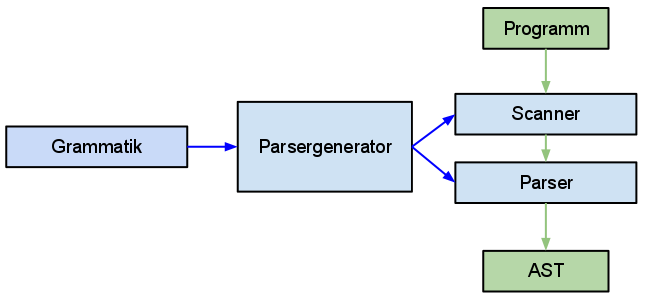
\includegraphics[scale=0.6]{figures/parser_generator_workflow}
\caption{Workflow eines Parser Generators (blau).}
\label{abb_parser_generator_workflow}
\end{figure}



\section{Vergleich}
\label{tools_vergleich}

Um eine Auswahl für die Implementierung des Interpreters zu treffen, ist es notwendig, die verschiedenen Tools anhand verschiedener Eigenschaften zu vergleichen. Das betrifft vor allem das Format der Grammatik und die vorhandenen Ein-/Ausgabesprachen.
Zusätzliche Faktoren sind die Werkzeugunterstützung (Grammatikeditor, Rule-Visualisierung, (Concrete/Abstract) Syntax Tree-Visualisierung), Dokumentation und (Community-)Support sowie Tools für den Build-Prozess.

In diesem Kapitel werden die Tools ANTLR, Coco/R und JavaCC verglichen. Diese sind alle für die Java-Plattform verfügbar und grundsätzlich für die in dieser Arbeit zu entwickelnde Sprache geeignet. Zusätzlich können diese Produkte als ausgereift betrachtet werden und wurden erfolgreich in verschiedenen Projekten eingesetzt.


\subsection{ANTLR}

Der Parsergenerator ANTLR wird von Terence Parr seit 1989 an der Universität von San Franzisco entwickelt und hat sich zu einem Quasi-Standard auf der Java Enterprise Plattform entwickelt. Unter anderem wird ANTLR im Applicationserver Weblogic, dem ORM-Mapper Hibernate, der IDE IntelliJ IDEA oder der JBoss Rules Engine Drools eingesetzt\footnote{vgl. http://www.antlr.org/showcase/list, 23.3.2012}.

ANTLR ist in Java implementiert, unterstützt aber diverse Zielsprachen wie Java, C++, C\#, Ruby, Objective C uvm. Für die Entwicklung steht eine ausgeprägte Palette an Tools zur Verfügung (siehe Abschnitt \ref{tools_antlr_tools}). Die Grammatik ist ein Format, das sich an der EBNF-Notation orientiert, aber erweiterte Konzepte wie Actions und Attribute zum Aufbau eines AST unterstützt. Lexikalische und Syntaktische Regeln können in seperaten Files abgelegt werden.

Neben der ausführlichen Dokumentation auf der Projektwebseite existiert auch ein Buch des Autors als Einfürung und Referenz\cite{Parr07}. Aufgrund der weiten Verbreitung in der Java-Welt steht ausreichend Support durch die Community zur Verfügung.



\subsection{Coco/R} 

Das Coco/R Projekt\cite{HaMo90} ist ein Parsergenerator, der ursprünglich von Hans\-peter Mössenböck an der Universität Linz entwickelt wurde. Zwischenzeitlich wurde das Projekt an der ETH Zürich fortgesetzt und ist inzwischen wieder an der Universität Linz beheimatet.

Coco/R ist nicht auf eine Plattform beschränkt und unterstützt diverse Sprachen. Es existieren Portierungen für u.A. Java, C++, C\# und VB.NET. Als Basis für die Angabe der Grammatik wird die EBNF-Notation verwendet. Angereichert wird diese durch Attribute und \emph{semantic Actions}. Durch diese Attribute kann ein AST aufgebaut werden\footnote{vgl. \cite{Moes11}}, allerdings muss dazu, im Gegensatz zu ANTLR, die ganze Grammatik abgeändert werden.

Auf der Homepage des Projkets steht ein ausführiches User Manual, sowie ausreichend Beispiele für jede Sprach-Portierung zum Download bereit. Zusätzlich bietet eine Mailingliste der Universität Linz Support. Es existiert ein Eclipse-Plugin für einen Grammatikeditor und die Erzeugung des Parsers beim Build.

\subsection{JavaCC}


JavaCC ist ein aus dem Sun-Projekt Jack entstandener Parsergenerator für die Java-Plattform. Auf der Projekthomepage wird er als ``the most popular parser generator for use with Java [tm] applications''\footnote{vgl. http://javacc.java.net/, 29.11.2011} bezeichnet. Eine Untermauerung für diese Behauptung, z.B. durch Projekte die JavaCC einsetzen, ist nicht zu finden. Laut Wikipedia\footnote{vgl. http://de.wikipedia.org/wiki/JavaCC, 29.11.2011} verwenden die Suchmaschine Lucene und das Ontologie-Framework Cyc durch JavaCC erstellte Parser.

Die Syntax wird in einer Grammatikdatei definiert, in der sowohl lexikalische als auch syntaktische Regeln angegeben werden. Die Ableitungsregeln enthalten zwei Blöcke: einen für die Ableitungsregel und einen für die Auswertung (sogenannte \emph{Action}) der Regel. Alternativ kann mithilfe des Tools JJTree ein Syntax-Baum erstellt werden.

Die Dokumentation ist recht ausführlich gestaltet. Für Support durch die Community steht eine Mailingliste zur Verfügung. Es gibt ein Eclipse-Plugin, das einen Code-Editor für JavaCC Grammatiken enthält. JavaCC ist in Java geschrieben und generiert Parser ausschließlich in Java.





\section{ANTLR}
\label{tools_antlr}
Dieser Abschnitt setzt sich im Detail mit ANTLR, dem Werkzeug der Wahl für diese Arbeit, auseinander. Wie bereits in Abschnitt \ref{tools_vergleich} erwähnt, sind alle angeführten Tools grundsätzlich für die DSL geeignet. Die entgültige Entscheidung für Entwicklung die Form Expression Language (FXL) ANTLR einzusetzen, begründet sich durch die hervorragende Dokumentation, insbesondere dem Buch des Autors, dem guten IDE Support und der Integration in das Build-Tool Maven.


\subsection{Grammatik}

Wie in Abschnitt \ref{tools_vergleich} erwähnt, orientiert sich das Format der Metasprache des Parsergenerators an der EBNF. Zusätzlich werden zusätzliche Angaben und Optionen in der Grammatikdatei gespeichert. Als Beispiel einer kompletten Grammatik kann jene der FXL im Anhang betrachtet werden.

\subsubsection{Optionen \& zusätzliche Angaben}

Es ist möglich, die Erzeugung von Parser und Lexer durch diverse Einstellungen zu beeinflussen.

\paragraph{Options}

Am Anfang eines Grammarfiles steht eine Auflistung von Parametern in einem \texttt{options}-Block. Diese steuern grundlegende Eigenschaften des generierten Parsers:

\begin{itemize}
  \item Ausgabesprache: Wie in Abschnitt \ref{tools_vergleich} erwähnt, beherrscht ANTLR diverse Ausgabesprachen. Hier muss angegeben werden, in welcher Sprache Lexer und Parser generiert werden sollen.

  \item Ausgabeformat: Das Format, das vom Parser beim Parsen eines Eingabestrings zurückgegeben wird. Dies kann entweder ein AST oder ein StringTemplate\footnote{StringTemplate ist eine Template Engine für verschiedene Einsatzbereiche. http://www.stringtemplate.org/, 23.3.2012} Template sein. Wird die Option weggelassen, wird nichts generiert, der Parser arbeitet dann als Recognizer, der nur den Eingabestring verarbeitet und im Fehlerfall eine Fehlermeldung ausgibt.

  \item Weitere Optionen: Weitere Optionen umfassen vor allem optimierende Parsingstrategien wie Memoizing und Backtracking (siehe Abschnitt \ref{theorie_erweiterte_konzepte}). Eine genaue Auflistung der Optionen befindet sich in der Re\-fe\-renz\cite{Parr07}.
\end{itemize}



\paragraph{Tokens umbenennen}

Literale können einfach als Strings, eingeschlossen in einfachen Anführungszeichen, in der Grammatik verwendet werden (siehe Listing \ref{listing_grammar_tree_compare}). Um diese Literal-Tokens im Interpreter besser verwenden zu können, bietet es sich an, diese mit sprechenden Namen zu benennen. Durch die Angabe \texttt{OR = 'OR';} im \texttt{tokens}-Block, wird im Parser automatisch eine Konstante \texttt{Parser.OR} generiert, auf die beim Abarbeiten des AST zugegriffen werden kann.

Weiters können auch Tokens erstellt werden, die in den Ableitungsregeln gar nicht vorkommen, aber für den Aufbau des AST benötigt werden. Ein Beispiel ist der \texttt{CALL}-Token in Listing \ref{listing_grammar_tree_function}, der beim Rewrite des AST verwendet wird (siehe folgender Abschnitt).

\subsubsection{Modellierung des Abstract Syntax Trees}

Würde man zur Weiterverarbeitung nach dem Parsen den Concrete Syntax Tree (CST) verwenden, würden die zahlreichen Knoten einen erheblichen Mehraufwand bedeuten. Deshalb ist es wichtig, wie der AST, der dann im Interpreter verwendet wird, aufgebaut sein soll. Dazu bietet ANTLR die Möglichkeit, in der Grammatik zu spezifizieren, wie der Baum aussehen soll. Das kann auf zwei Arten geschehen: inline oder explizit als Rewrite-Regel.

Bei der Inline-Angabe (Listing \ref{listing_grammar_tree_compare}) wird nur jenes Element (Literal, Terminal, oder Nonterminalsymbol) ausgewählt, welches als Wurzelelement des AST-Knotens gewählt wird. Die übrigen Elemente werden in der Reihenfolge ihres Auftretens als Kindelemente angehängt. Elemente, die im AST ignoriert werden sollen, weil sie in der Baumdarstellung ihre Relevanz verlieren (z.B. Klammern, Trennzeichen etc.), werden mit einem Rufzeichen markiert und nicht als Kindelement zum Knoten hinzugefügt.


\begin{lstlisting}[float = htbp,caption={Inline-Regeln zur Beschreibung der Baumstruktur.},label=listing_grammar_tree_compare]
compareExpression
  	:
  	commonExpr (('<'|'>'|'='|'<='|'>='|'!=')^ commonExpr)?
  	;

\end{lstlisting}

Rewrite Regeln können die Baumstruktur auch stark verändern und Knoten einführen, die als solches nicht in der Regel vorkommen. Dazu wird die Regel wie in Listing \ref{listing_grammar_tree_function} einfach an die rechte Seite der Ableitungsregel angehängt. Nun kann der Knoten für diese Regel im Format \texttt{\textasciicircum(Root Child1 ... Childn)} angegeben werden, wobei Root den Tokentyp des AST-Knotens bezeichnet, gefolgt von den Kindknoten. 


\begin{lstlisting}[float = htbp,caption={Rewrite-Regeln zur Beschreibung der Baumstruktur.},label=listing_grammar_tree_function]
functionCall
  :
  ID '(' arguments ')' -> ^(CALL ID arguments?)
  ;
\end{lstlisting}

Im Beispiel in Listing \ref{listing_grammar_tree_function} wird der Tokentyp \texttt{CALL} als Typ des Knotens festgelegt. Dazu muss dieser Token allerdings zuerst im Token-Abschnitt des Grammarfiles festgelegt werden (siehe oben). Als erstes Kindelement wird ein Knoten vom Typ \texttt{ID} erstellt, der den Namen der Funktion enthält. Die weiteren Kindknoten sind die optionalen Argumente, wobei diese wiederum komplexe Ausdrücke in Form von Subtrees enthalten können (siehe FXL-Grammatik im Anhang).

\begin{figure}[h]
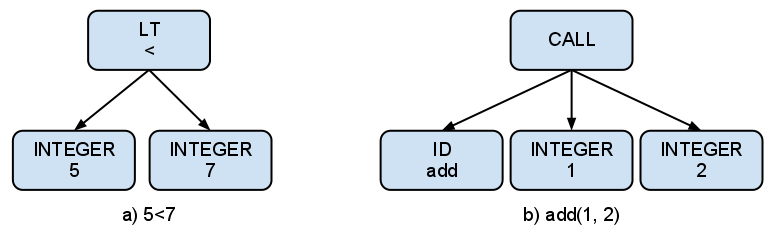
\includegraphics[scale=0.5]{figures/ast_beispiele}
\caption{a) Aufbau des AST bei Inline-Notation. b) Aufbau des AST bei Rewrite-Notation}
\label{abb_ast_beispiele}
\end{figure}

Abbildung \ref{abb_ast_beispiele} Zeigt jeweils ein Beispiel für die zwei Tree-Building Methoden. Die Knoten enthalten jeweils den Tokentyp und den Text des Knotens. In Beispiel a) wird das Kleiner-Zeichen als Wurzelelement verwendet, die anderen Elemente werden als Knoten vom Typ Integer als Kindknoten angehängt. Beispiel b) zeigt den Sonderfall des künstlichen Tokens \texttt{CALL} aus Listing \ref{listing_grammar_tree_function}, der nur zum Umformen des Baumes verwendet wird.


\subsection{Tools}
\label{tools_antlr_tools}

Werkzeuge können den gesamten Entwicklungsprozess effizienter und einfacher gestalten. Sei es durch Tools wie einem Editor oder Debugger bei der Programmierung, oder solche zur Automatisierung des Buildprozesses. Vor allem Integrierte Entwicklungsumgebungen (IDEs) unterstützen den Entwickler beim Design einer Sprache. Im Falle eines Parsergenerators besteht eine IDE aus einem guten Editor für die Grammatik (Syntax Highlighting, Code Completion etc.), visuellen Darstellungen der Grammatik und einzelner Regeln, sowie einer Testumgebung zur Evaluierung der Syntax.

\subsubsection{ANTLRWorks}

ANTLRWorks \footnote{vgl. http://www.antlr.org/works/index.html, 23.3.2012} ist ein Tool zum Entwickeln von Grammatiken für ANTLR. Es ist in vielerlei Hinsicht eine Hilfestellung, da es vor allem visuelle Hilfestellungen, wie Syntaxdiagramme oder Syntaxbäume, bietet. Der Hauptteil von ANTLRWorks besteht aus dem Grammatikeditor und der Auflistung der Grammatikregeln. Der Editor selbst bietet einige Features, die von anderen IDEs bekannt sind wie etwa Syntax Highlighting und Code Completion.

\begin{figure}[h]
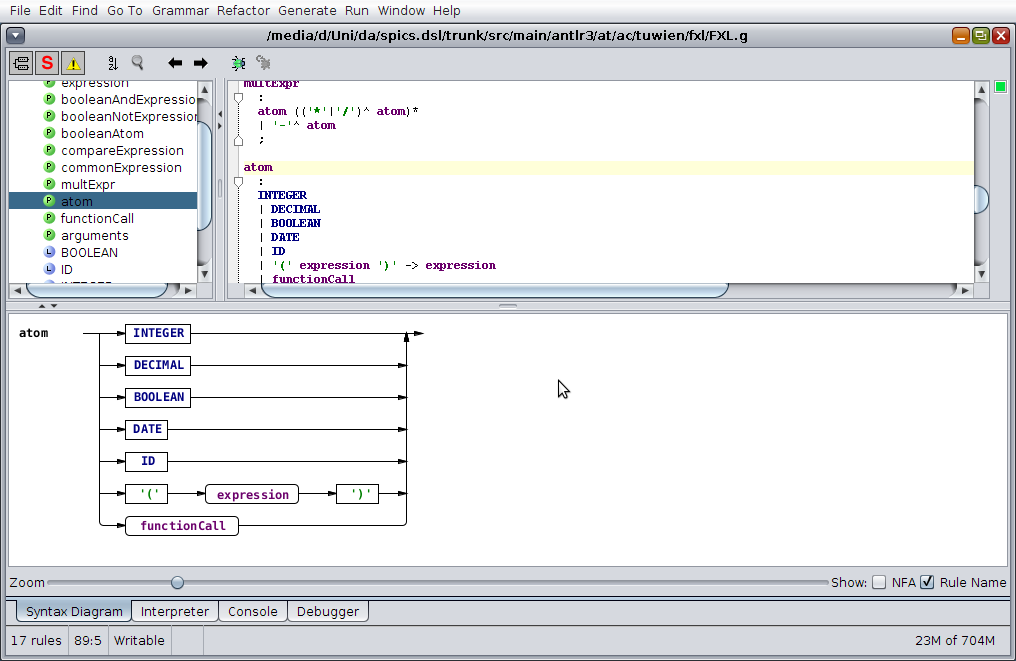
\includegraphics[scale=0.35]{figures/antlrworks_syntax_diagram}
\caption{Syntax Diagram in ANTLRWorks}
\label{abb_antlrworks_syntax_diagram}
\end{figure}

Ein weiteres Feature ist die Darstellung der Regeln in Syntaxdiagrammen (Abbildung \ref{abb_antlrworks_syntax_diagram}). Syntaxdiagramme werden dazu verwendet, Grammatiken graphisch darzustellen. Insbesondere können einzelne Regeln, die textuell durch Verzweigungen und Wiederholungen recht schnell komplex werden, mit Hilfe von Syntaxdiagrammen recht einfach nachvollzogen werden.

\begin{figure}[h]
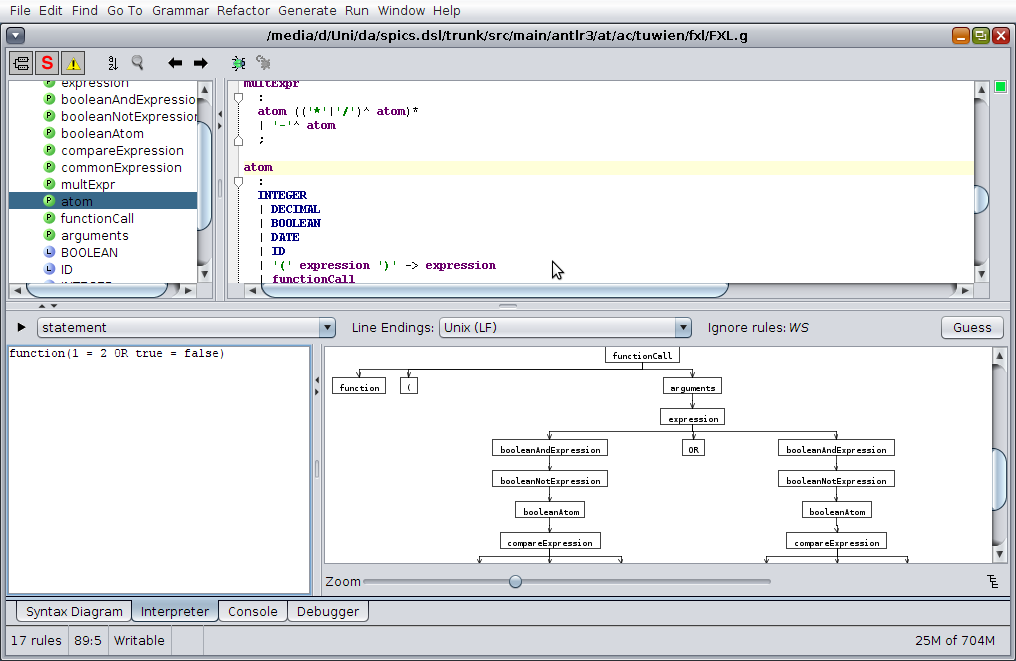
\includegraphics[scale=0.35]{figures/antlrworks_interpreter}
\caption{Interpreter/Concrete Syntax Tree in ANTLRWorks}
\label{abb_antlrworks_interpreter}
\end{figure}

ANTLRWorks kann auch beliebige Eingabestrings parsen und gegen die verschiedenen Ableitungsregeln testen. Der resultierende Parsebaum wird graphisch dargestellt. Tritt ein Fehler auf, so wird das Parsen unterbrochen und die Stelle im Parsebaum, an der der Parser nicht fortsetzen kann, markiert. Auf diese Art können nicht nur Statements die von der Startregel ausgehen getestet werden, sondern auch Eingaben für beliebige Unterregeln.


\begin{figure}[h]
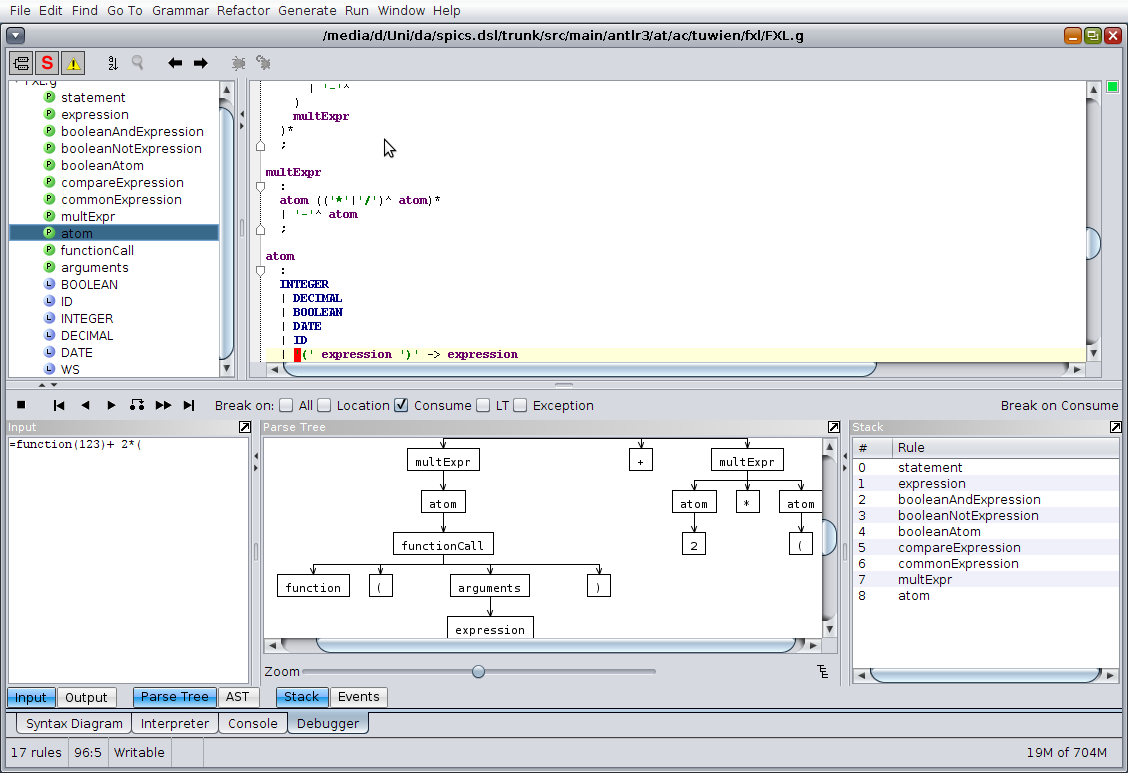
\includegraphics[scale=0.35]{figures/antlrworks_debugger}
\caption{Der Debugger von ANTLRWorks}
\label{abb_antlrworks_debugger}
\end{figure}

Ein Key-Feature von ANTLRWorks ist der Debugger (Abbildung \ref{abb_antlrworks_debugger}). Mit Hilfe des Debuggers lässt sich der Parseprozess Schritt für Schritt nachvollziehen. Während des Parsens wird für jeden Schritt angezeigt, welche Regel gerade angewendet wird. Zusätzlich wird der Parsebaum im mittleren Fenster schrittweise aufgebaut.

ANTLRWorks beherrscht sogar das Debuggen von Parsern in anderen Sprachen. Dies ist möglich, da ANTLRWorks per Sockets mit dem Parser kommuniziert\footnote{ vgl. http://www.antlr.org/works/index.html, 23.3.2012}.


ANTLRWorks ist ein mächtiges Werkzeug, das den Entwickler effektiv bei der Entwicklung von Grammatiken unterstützt. Der Nachteil ist jedoch, dass es ein eigenständiges Tool ist, dass zusätzlich zu diversen anderen Tools in den Entwicklungsprozess eingebunden werden muss. Für eine bessere Integration in diesen stehen diverse IDE-Plugins zur Verfügung, die im folgenden Abschnitt behandelt werden.
 
\subsubsection{IDE-Plugins}

Mittlerweile existieren diverse Plugins für die wichtigsten Entwicklungsumgebungen\footnote{Eine aktuelle Übersicht über die Plugins für diverse IDEs findet sich unter http://www.antlr.org/wiki/display/ANTLR3/Integration+with+Development+Environments}. Für IntelliJ IDEA existiert ein Plugin, das ANTLRWorks direkt in die IDE integriert. Der Funktionsumfang ist dementsprechend gleich umfangreich wie ANTLRWorks selbst.

Für die weit verbreitete offene IDE Eclipse existieren zwei Plugins. AntlrDT stellt vor allem einen Code-Editor und die Integration in den Eclipse Buildprozess (automatisches Compilieren nach Clean bzw. Speichern) zur Verfügung. Zusätzlich bietet das Plugin auch die Visualisierung von ASTs an, die allerdings, im Vergleich zu ANTLRWorks, nicht so ausgereift erscheint. Das zweite Eclipse-Plugin ist ANTLR IDE\footnote{http://antlrv3ide.sourceforge.net/, 23.3.2012}. Es ist sehr ausgereift und wurde auch für die Implementierung der Form Expression Language in der vorliegenden Arbeit verwendet. Es bietet einen Grammatikeditor, eine Ansicht für Syntaxbäume (im Plugin Railroad View genannt) und einen Interpreter, mit dem wie in ANTLRWorks Eingaben auf verschiedene Regeln angewendet werden können. Auch ein Debugger ist vorhanden, der allerdings im Gegensatz zu ANTLRWorks nur mit Java-Parsern arbeiten kann.

\subsubsection{Build Tools} 

Alle oben genannten Plugins integrieren ANTLR in den Buildprozess der Entwicklungsumgebung. Für ANTLR bedeutet dies, dass Lexer und Parser automatisch beim Build der Software aus der Grammatik generiert wird. Oft wird allerdings ein externes Tool zum Build bzw. zur Auslieferung von Software verwendet. Für die zwei verbreitetsten Buildtools auf der Java-Plattform, Apache Ant und Apache Maven, existieren Erweiterungen, die die Codegenerierung übernehmen\footnote{vgl. http://www.antlr.org/wiki/display/ANTLR3/How+to+use+ant+with+ANTLR3 bzw. http://www.antlr.org/antlr3-maven-plugin/index.html}.



\chapter{Related Work}
\label{related_work}

In diesem Kapitel wird eine Übersicht über das wissenschaftliche Umfeld dieser Arbeit geboten. Einige der vorgestellten Ansätze und Projekte gaben Anregungen für die Form Expression Language, die in dieser Arbeit entwickelt wurde. Es lassen sich zwei Bereiche identifizieren, die dem Umfeld der Arbeit entsprechen. Einerseits verschiedene Sprachen zur Berechnung und Evaluierung von Werten sowie DSLs zur Modellierung von Webformularen. Die Themen Domain Specific Languages und Parser Generatoren wurden bereits weiter oben behandelt.

\section{Sprachen zur Berechnung und Evaluierung von Werten}

Eine Sprache, die sich in wissenschaftlichen Arbeiten oft wiederfindet, ist die Object Constraint Language (OCL)\cite{RiGo98}.Die Object Constraint Language (OCL) ist ein Teil der UML - Spezifikation und wurde ursprünglich für die Modellierung von Klassen- und Sequenzdiagrammen angedacht. Ein weiterer Einsatzort ist die Modellgetriebene Entwicklung. Dort wird OCL etwa im Bereich Transformation von (Meta-) Modellen und Modelchecking verwendet\footnote{vgl. http://www.eclipse.org/modeling/mdt/?project=ocl, 21.3.2012}. Escott et al.\cite{Esco12} setzen die OCL zur Validierung von Webformlaren ein (siehe unten).

Eine weitere Sprache, die einfache Berechnungen und Validierungen ermöglicht, ist die Unified Expression Language (UEL). Diese ist aus den sehr ähnlichen Expression Languages für JavaServer Pages(JSP) und JavaServer Faces(JSF) entstanden. Die UEL kann auf Java-Objekte zugreifen, Werte setzen beziehungsweise abfragen und Methoden aufrufen. Eine freie Implementierung ist JUEL\footnote{http://juel.sourceforge.net/, 21.3.2012}. JUEL hat den Vorteil, dass sie außerhalb des Java Server Kontexts für beliebige Anwendungsgebiete verwendet werden kann.

Auf der Java-Plattform entstanden verschiedene Implementierungen von Skriptsprachen, die innerhalb der Anwendung ausgeführt werden können. Zwei der bekanntesten Projekte sind Mozillas JavaScript-Engine Rhino\cite{wwwRhino} und die Python und Ruby Portierungen Jython bzw. JRuby. Der Java Specification Request JSR-233 definiert eine standardisierte API \cite{JSR-223}, um Skripte in einer Java Anwendung auszuführen und Java-Objekte an die Engine zu binden\footnote{vgl. Abschnitt \ref{section_java_scripting}}.  Seit Java 1.6 stehen einige Scriptengines out-of-the-box zur Verfügung, u.a. JavaScript, Groovy und Ruby. Programme in Form von Skripts können zur Runtime erstellt und verändert werden. Es können Variablen an die Engine übergeben und im ausführenden Skript verwendet werden. Zusätzlich kann auf die gesamte Java API zugegriffen werden. Nach der Ausführung kann wiederum auf die Variablen zugegriffen werden. 

Zuletzt sollen noch die Formelsprachen von Tabellenkalkulationswerkzeugen wie Microsoft Excel oder LibreOffice Calc Erwähnung finden, da diese ein Vorbild für die Syntax der FXL sind.


\section{DSLs zur Modellierung von Formularen}

Der Wunsch nach erweiterten Möglichkeiten zur Modellierung von Web Formularen ist nicht neu. Dieser Wunsch äußert sich in verschiedenen Ansätzen, Webanwendungen allgemein und Formulare im Speziellen semantisch anzureichern. Die verschiedenen Ansätze weisen unterschiedlichen Stärken und Schwächen auf. In diesem Abschnitt wird auf verschiedene Arbeiten in diesem Gebiet eingegangen.

Eine Schwierigkeit besteht darin, dass Web-Applikationen in eine Client- und eine Serverseite aufgeteilt sind, wobei der Client meistens nicht vertrauenswürdig ist. Anwendungen der Clientseite (vor allem mit HTML und JavaScript) können durch deren offene Natur leicht manipuliert werden. Berechnungen und Validierungen im Client können also nicht als sicher angesehen werden, eine zusätzliche Überprüfung auf dem Server ist also notwendig. 

Zwei Ansätze, die auf Kosten der Offenheit versuchen, die Manipulierbarkeit von Anwendungen in den Griff zu bekommen, sind Adobe Flash (bzw. Flex und Air) und Java Applets (bzw. JavaFX). Diese setzen allerdings, im Gegensatz zu den gängigen Technologien HTML und JavaScript, die mit verschiedenen Clients funktionieren, mehr oder weniger proprietäre Laufzeitumgebungen für die Applikationen vorraus.

Ein Ansatz für eine DSL zur Modellierung von Formularen, ist das Projekt Mawl der Bell Laboratories\cite{AtBa99}. Mawl ist eine DSL für ``Form-based services''mit der aus HTML-Templates und der Programmlogik in der DSL Webanwendungen entwickelt werden können. Die Applikation wird zu Skripts für die CGI Schnittstelle kompiliert. Als Nachfolger von Mawl gilt das Projekt Bigwig\footnote{http://www.brics.dk/bigwig/, 15.3.2012}, ein Framework zur ``Entwicklung von interaktiven Web Services''. Bigwig-Programme werden in C-Code, HTML und JavaScript umgewandelt. Das Framework bietet Komponenten für verschiedene Apekte wie dynamische Dokumente, Security, Datenbankanbindung und Validierung von Eingaben, PowerForms genannt. Der Ansatz von Powerforms\cite{BrMo00} ist eine deklarative DSL im XML-Format, um HTML-Formulare durch Constraints zu erweitern. Die Constraints können, wie in dieser Arbeit gefordert, auch andere Formularfelder referenzieren. Der Nachfolger JWIG ist als allgemeines Web-Application Framework zu betrachten, ohne explizite Features einer DSL.

Ein weiterer Ansatz, der erweiterte Modellierungen von Webformularen ermöglicht, ist XFORMS. XFORMS ist ein W3C-Standard\cite{Xfor09}, der die detaillierte Modellierung von Formularen zum Ziel hat. Formulare können clientseitig durch diverse Constraints, Validierungen und Berechnungen erweitert werden. Durch das \texttt{calculate} Attribut werden Berechnungen mit Werten anderer Felder ermöglicht\cite{Chas07}. XFORMS wäre Teil des XHTML 2.0 Standards gewesen, der sich allerdings gegen HTML 5 nicht durchsetzen konnte.

WebEAV\cite{NaPr00} ist ein Framework zur Metadaten-gesteuerten Generierung von Webformularen für Entity-Attribute-Value Datenbanken. Metadaten beschreiben, wie einzelne Formulare zusammengesetzt werden sollen. Es ist möglich, Constraints und Abhängigkeiten zu definieren, die auf der Clientseite berechnet werden. WebEAV generiert Scripts, die Abhängigkeiten zwischen den Feldern beschreiben. Die Berechnungen im Browser erfolgen mit der JavaScript Funktion \texttt{eval()}, die Programmcode als Script entgegennimmt und ausführt. Wie in dieser Arbeit können jene Felder, die von einer Berechnung beeinflusst werden, ebenfalls neu berechnet werden.

Escott et al.\cite{Esco12} entwerfen einen Anzatz für die modellgetriebene Entwicklung, in dem UML-Modelle mit zusätzlichen Informationen angereichert werden. Drei Typen von Validierungen werden identifiziert: \emph{Single element}, \emph{Multiple element} und \emph{Entity association}. \emph{Single element} bezeichnet Validierungen, die sich auf das Element selbst beziehen, also beispielsweise Beschränkung der Werte auf minimale oder maximale Schranken. \emph{Multiple element} bezieht sich auf Felder, die von anderen Feldern abhängig sind. Diese Constraints werden dem Modell als OCL-Ausdrücke hinzugefügt. Der dritte Typ, \emph{Entity associations}, validiert die Multiplizitäten des UML-Modells.

WebDSL\cite{Vis08} ist eine DSL für die Entwicklung von Webanwendungen. Die Elemente einer Applikation, etwa Datenmodell, User Interface, Benutzerinteraktionen und Zugriffskontrolle werden in einem sehr hohen Abstraktionsgrad beschrieben. Der DSL-Code wird in eine Java Webanwendung übersetzt und auf dem Servlet Container Tomcat deployed. Ein Teil der WebDSL ist die Integration der Datenvalidierung\cite{GrVi09} auf verschiedenen Ebenen: Überprüfen von Werten und Typen, Constraints des Models, Model-unabhängige Constraints, sowie Constraints beim Bearbeiten eines Formular-Requests. Für die letzten drei Ebenen können boolesche Ausdrücke erstellt werden, die auf Daten des Requests und des Models zugreifen können.


